En esta sección se presenta la solución escogida
para mejorar la problemática de las pequeñas empresas para competir en lo
referente a comercio electrónico con sus pares mayores.

\section{Metodología de la solución}
\label{sec:4.1}

Para dar solución a la problemática de las micro empresas,
que consiste en atraer y retener clientes, para así poder competir
con empresas de mayor tamaño, tiene como base el uso de una herramienta
OpenSource, para así crear una tienda virtual atractiva a los usuarios
y que pueda estar a la altura de grandes sitios web.

Las siguientes características son necesarias para poder implementar un sistema
web enfocado a una pequeña empresa, que no posee los recursos necesarios
para un gran despliegue web:

\begin{itemize}
    \item {\bf Bajo costo:}
        Debido al bajo capital que poseen estas empresas, el costo
        es bastante crucial.
        La poca viabilidad de utilizar soluciones completas ofrecidas
        por empresas externas, lleva a utilizar una o más herramientas
        que en su conjunto emulen a un sistema completo que necesita ser
        implementado.

    \item {\bf Facilidad de configuración:}
        Existen diversas herramientas que ayudan a un negocio emergente a crear
        una sitio web, pero pocas están pensadas para ser configuradas y administradas
	por un usuario sin tantos conocimientos tecnológicos.
        Esta característica es vital, pues como ya mencionamos,
        se necesita una persona con los conocimientos necesarios tanto
        de instalación como configuración, los cuales pueden ser solucionados
        con la contratación de una persona externa.

    \item {\bf Facilidad de administración:}
        Característica clave dentro de la solución planteada.
        El sistema será administrado, la mayoría del tiempo, por el dueño de la
        empresa, el cual debe ser capaz de realizar tareas en el sistema
        de manera rápida y frecuentemente, por lo que un grado
        de complejidad en términos de administración jugarán en contra
        a la hora de poder aprovechar el sistema a disposición.
        Adicionalmente, se necesita un sistema de administración rápido,
        para evitar estar mucho tiempo realizando una tarea simple, que
        además de conocimientos del sistema, pueden ser provocados por sistemas
        que no poseen una implementación de funcionalidades ordenadas.

\end{itemize}

Una vez creada la tienda virtual, la empresa entra a competir electrónicamente,
pero en desventaja, con empresas de mayor capital, y por ende, con tiendas virtuales
de mayor tamaño que utilizan conceptos para atraer y retener a los clientes.
Para competir directamente, es necesario utilizar estos mismo conceptos para
poder alcanzar, de cierta forma, el nivel de visitas y ventas de estos grandes
sitios web.

Para ayudar a disminuir la brecha entre la solución propuesta y una tienda virtual
de gran tamaño utilizaremos el concepto de {\GAM}.
Este concepto ayudará a la tienda a atraer y retener clientes con la utilización
de elementos de los juegos, que ya se han mencionado en este documento,
de los cuales se han seleccionado los siguientes elementos, como parte
de un esquema clave a implementar. Estos ya han sido utilizados y probados en diversos
sistemas como herramientas para motivar al usuario\cite{SocialMotivation}

\begin{itemize}
    \item {\bf Puntuación:}
	Este estilo de recompensa es uno de los primeros creados como parte de
	implementar {\gam}. Es una de las formas más sencillas de empezar
 	a utilizar {\gam}\cite{OnlineComp} y de la cual se pueden basar 
	otros tipos de recompensas,
	vease figura \ref{fig:ranking}.

        En el contexto de nuestra solución, esta herramienta consiste en la entrega de
	puntos por la realización de tareas definidas, como:

    \begin{itemize}
        \item Inscripción:
            Esta tarea otorga al usuario 500 puntos.
        \item Comentarios en productos:
            Otorga 100 puntos por cada comentario, con un máximo de 5 comentarios
            con premio.
        \item Compras realizadas:
            Se le premia con un 10\% de la compra en puntos.
    \end{itemize}

        Estos puntos son equivalentes a crédito en la tienda y pueden ser
        utilizados como parte de pago.
        Son utilizados para que los clientes vuelvan a comprar a la tienda,
        utilizando créditos generados por él mismo.

\begin{figure}[!htb]
  \centering
  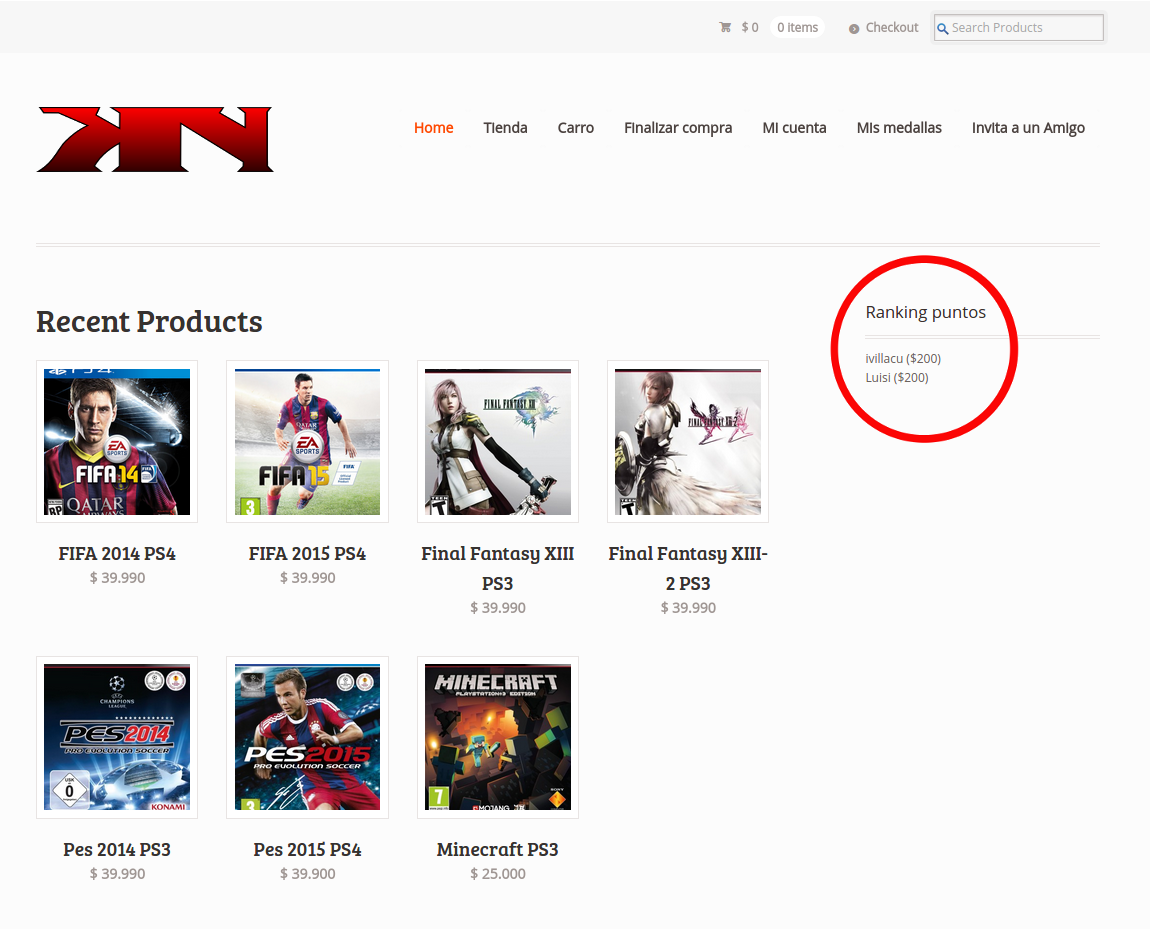
\includegraphics[width=0.9\textwidth]{images/Tienda/Tienda_ranking.png}
  \caption[Ranking puntos]{Utilización de puntos en ranking.}
  \label{fig:ranking}
\end{figure}


    \item {\bf Achievements (logros):}

	Esta forma de motivación, a través de la entrega de medallas o \emph{achievements}
	ha empezado a ser utilizada para manejar el comportamiento de los
	usuarios dentro de la web\cite{BehaviorBadges}.

        Dentro de la solución se implementará la entrega de medallas (\emph{achievements})
	coleccionables entregada a los clientes por cumplir con tareas definidas, vease
	figura \ref{fig:achievement}, como:

        \begin{itemize}
            \item Inscribirse.
            \item Primer inicio de sesión.
            \item Primer comentario/reseña.
            \item Primera orden completada.
            \item Compra por una suma mayor a \$15,000 CLP.
        \end{itemize}

        Esta recompensa es utilizada con el fin de entregar la sensación de éxito,
        e importancia entre otros compradores y así mantener una motivación
        de seguir comprando y su estado dentro de la comunidad.

\begin{figure}[!htb]
  \centering
  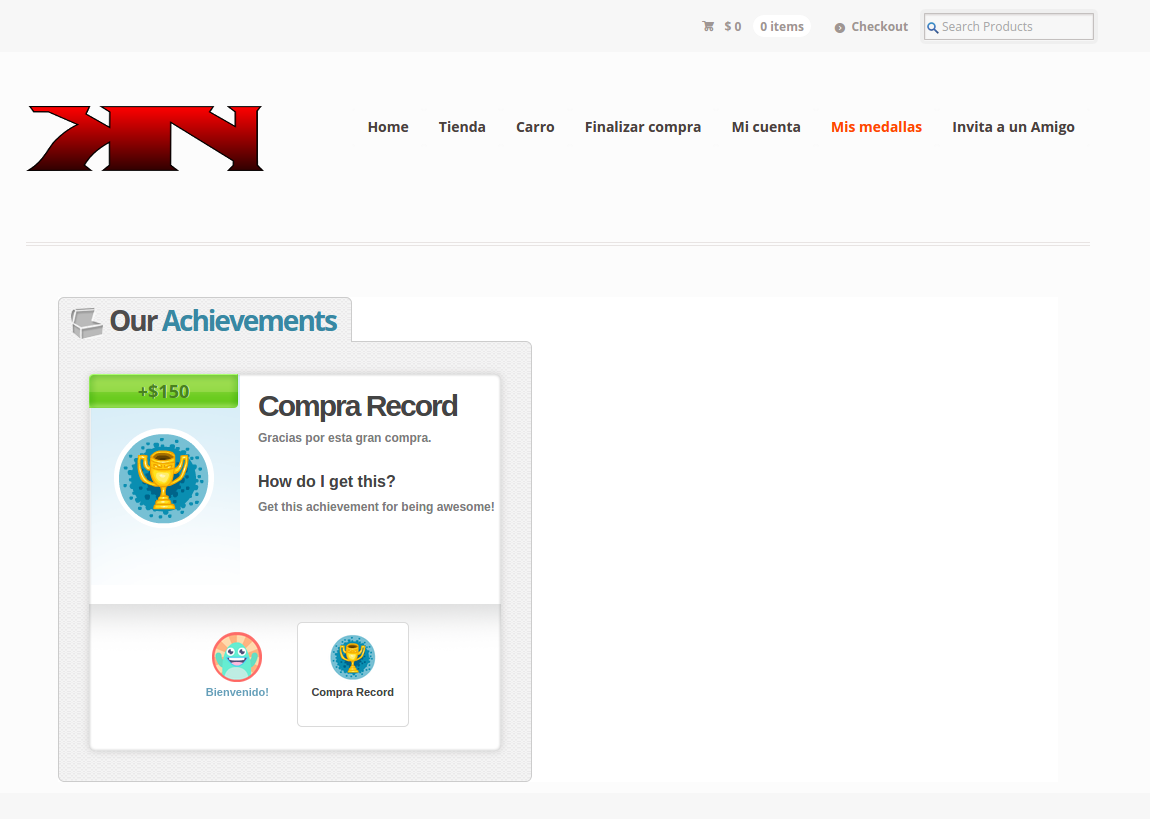
\includegraphics[width=0.9\textwidth]{images/Tienda/Tienda_achievement.png}
  \caption[Achievement]{Achievements del sistema.}
  \label{fig:achievement}
\end{figure}



    \item {\bf Referals (Referencias):}
        Invitaciones de usuarios de la tienda que son entregadas a posibles
        clientes para que estos conozcan y compren en la tienda, vease figura 
	\ref{fig:referal}.
        Esta herramienta entrega un beneficio mutuo tanto al que hizo la invitación
        como al invitado. Esta recompensa es un cupón de descuento de 500 puntos.
        En primer, lugar el usuario invita a un cliente no suscrito en la tienda
        enviando un cupón válido por 500 puntos.
        Luego, éste al comprar con este cupón reenvía,
        proceso interno, un cupón de 500 puntos al usuario que lo invitó.
        Esto es utilizado para atraer clientes con gustos similares
        a la tienda, pues el usuario que entregue invitaciones, lo hará a su
        grupo cercano, y así sucesivamente.

\begin{figure}[!htb]
  \centering
  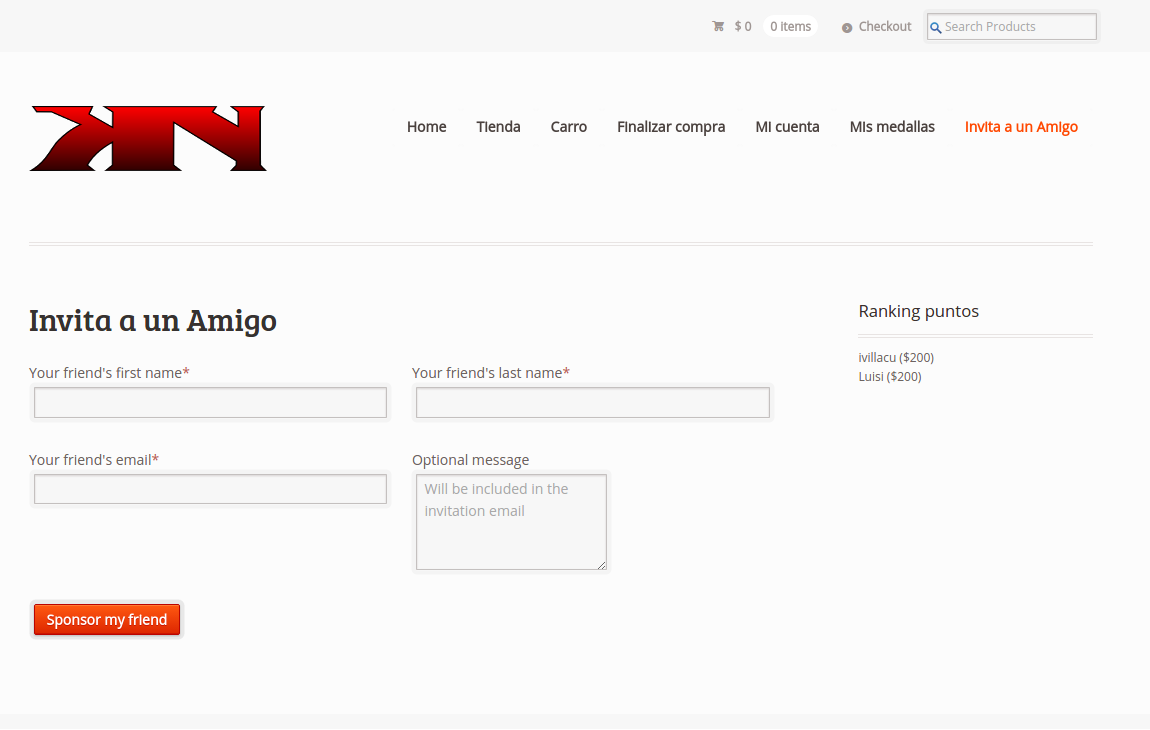
\includegraphics[width=0.9\textwidth]{images/Tienda/Tienda_referal.png}
  \caption[Referal]{Refer a Friend del sistema.}
  \label{fig:referal}
\end{figure}

\end{itemize}

Al unir la tienda virtual con las ideas propuestas dadas por {\gam}, se crea un
sistema de ventas \emph{on-line} capaz de competir con las características similares del
comercio electrónico de tiendas que poseen más capital y experiencia en este ámbito.

\section{Selección de sistema}

Como parte de la investigación, se tuvieron que seleccionar distintos sistemas web para
crear una tienda electrónica, estos son \emph{Magento}, \emph{Prestashop}, \emph{Wordpress
$+$ Woocommerce}.

Para poder elegir entre estos sistemas, se proponen las siguientes métricas:

\begin{itemize}

    \item {\bf Facilidad de instalación:}
        Esta métrica muestra el nivel de conocimientos que se debe
        tener para poder realizar una instalación completa y exitosa del sistema.
        También demuestra que tanta ayuda existe durante la misma (comentarios,
        ejemplos, etc).
        Ésta se medirá con una escala de uno(1) lo más fácil a diez(10) lo más difícil.

    \item {\bf Facilidad de administración:}
        Escala que mide el nivel de conocimientos para poder utilizar el
        \emph{dashboard} de administración de cada sistema.
        También se toma en cuenta la ayuda y ejemplos que da el sistema al usuario.
        Esta medida en una escala de uno(1) a diez(10), siendo uno(1) el más fácil y diez(10) 
	el más difícil.

    \item {\bf Actualizaciones y comunidad activa:}
        Métrica que demuestra que tan periódicamente se realizan actualizaciones
        al sistema.
        También mide la comunidad que existe tras cada proyecto tanto en tamaño
        como en actividad.
        Esta escala también se mide entre uno(1) y diez(10), siendo uno(1) una periodicidad 
	alta de actualizaciones y una comunidad altamente activa
	y 10 una periocidad baja y falta de comunidad.

    \item {\bf Características utilizables:}
        Mide la existencia de plugins que implementen herramientas de {\GAM}
        y si éstas son gratuitas o de pago.
        Si son de estas últimas, si son de bajo o alto costo.

    \item Traducciones:
        Muestra si existe una traducción del sistema a otros idiomas, en especial
        al español.

\end{itemize}

En el siguiente cuadro~\ref{tab:comp_tools} muestra la comparación de los tres
sistemas preseleccionados para implementar la solución propuesta.

\begin{table}[h]
\footnotesize
\setlength\extrarowheight{5pt}
\begin{tabular}{| p{2.5cm} | p{1.8cm} | p{2.5cm} | p{2.8cm} | p{2.5cm} | p{2cm} |}
\hline
                        & Dificultad de\newline Instalación
                        & Dificultad de\newline Administración
                        & Actualizaciones y\newline Comunidad
                        & Características\newline Utilizables
                        & Traducción \\ \hline

Magento                 & 7 & 8 & 8 & Si tiene plugins,\newline Alto costo & Parcialmente \vspace{0.2cm} \\ \hline
Prestashop              & 6 & 7 & 9 & No tiene plugins                     & Si    \vspace{0.2cm}\\ \hline
Wordpress +\newline Woocommerce & 4 & 5 & 2 & Si tiene plugins,\newline Gratuitas,\newline Bajo costo,\newline Alto Costo & Si\\ \hline
\end{tabular}
\caption{Tabla de comparación entre los sistemas bases investigados}
\label{tab:comp_tools}
\end{table}

\section{Herramientas}

Para implementar la solución propuesta se utilizan diferentes herramientas.
En un principio se penso en el desarrollo completo de las
tareas requeridas, pero luego de investigar el estado del arte de estas tecnologías,
se tomó la decisión de utilizar herramientas ya disponibles que tuviesen
características similares a las requeridas en donde su modificación requeriría
menos tiempo que el desarrollo completo.
Otra característica que ayudó al cambio de paradigma fue que en todas las
herramientas a utilizar, existe una comunidad altamente activa que da soporte y que
llegaría a ser útil al momento de configurar o modificar alguna de éstas.

La base del sistema utilizado es Wordpress, por ser uno de los
CMS~\footnote{Content management system o Sistema de gestión de contenidos}
más famosos, y ampliamente utilizado\cite{CmsPerformance}.

Esta herramienta permite crear una web para manejar contenidos de una forma fácil,
tanto la instalación como la administración de las funcionalidades básicas del sistema.

Wordpress posee una fase de instalación sencilla debido a que los recursos
necesarios son pocos. Se necesita poseer un \emph{hosting} donde alojar el sitio y
dominio, además de una base de datos relacional, como MySQL o PostgreSQL, que en la mayoria
de las ocaciones es ofrecida por el mismo hosting.
Una gran ventaja de esta herramienta es que al necesitar recursos básicos,
servidor web y base de datos relacional, puede ser instalado de manera fácil en la
mayoría de los \emph{hostings} a nivel mundial.
Una vez instalado, la administración total del sistema es relativamente simple,
ya que posee un \emph{dashboard} con todas las opciones necesarias
tanto para la configuración inicial del sistema, como para la modificación
de algunas características importantes, desde el contenido, hasta el tema
y diseño del sitio.

Las características principal de Wordpress, que ha ganado mediante
la comunidad detrás del proyecto, es la variedad de plugins, que
tienen tanto un proceso de instalación fácil, como su administración,
la cual sigue los mismos principios de administración de Wordpress.
Dichos plugins, son el elemento distintivo de cada CMS
y en nuestro caso, han sido los actores principales para aplicar
todos los elementos de {\GAM} en el sistema web.

\begin{figure}[!htb]
  \centering
  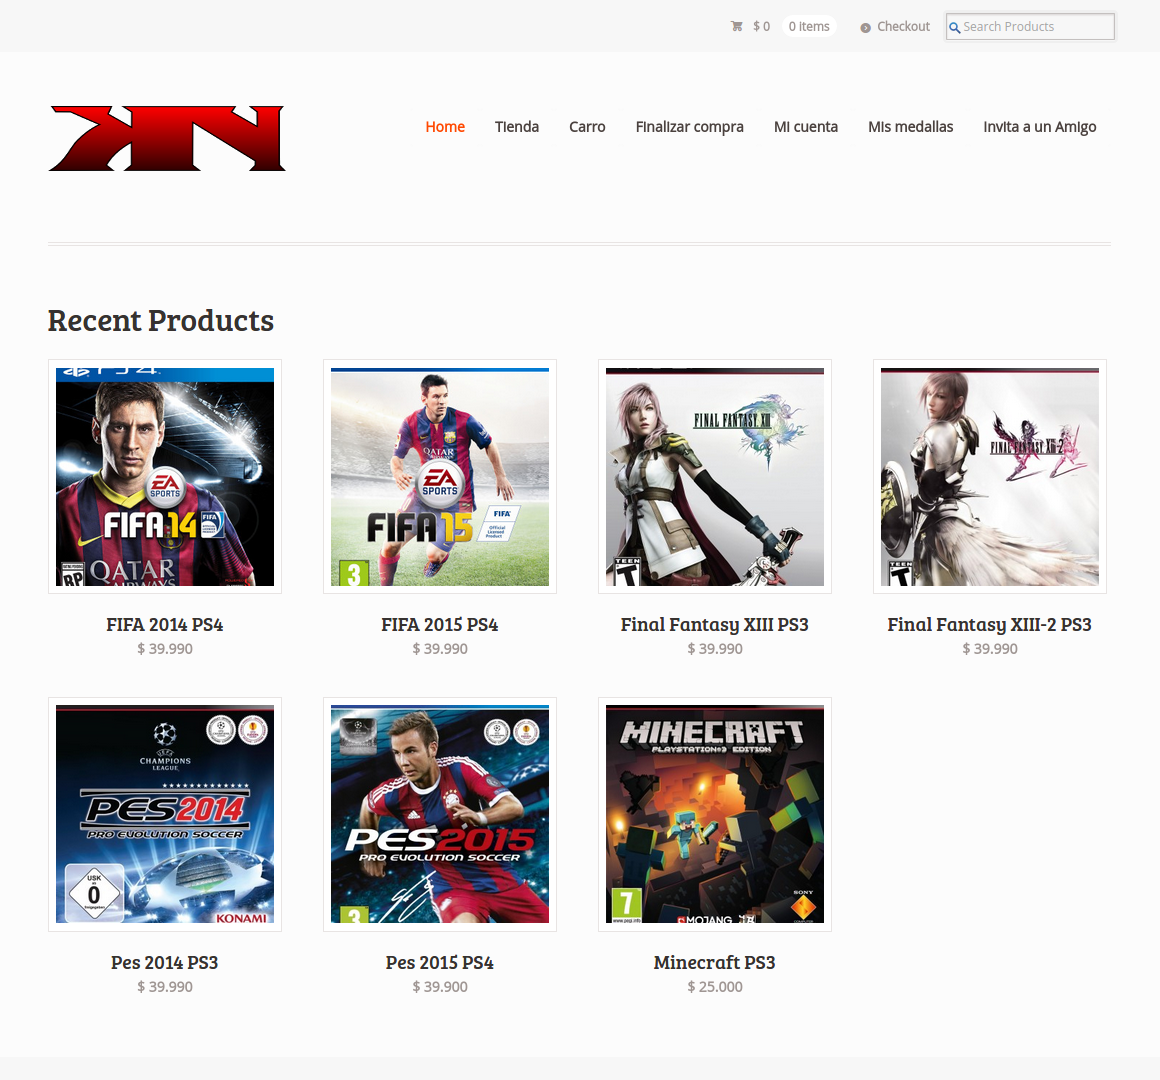
\includegraphics[width=0.9\textwidth]{images/Tienda/Tienda.png}
  \caption[TemaVisual]{Tema visual utilizado, vista de la tienda.}
  \label{fig:Players}
\end{figure}



Los plugins utilizados en nuestro sistema, son los siguientes:

\begin{itemize}

    \item {\bf Woocommerce:}
        Es un reconocido módulo que ayuda al usuario a crear una tienda de
        ventas \emph{on-line} de forma rápida y sin costo.
        Al ser integrado al sistema, lo modifica agregando opciones
        extra de configuración y administración.
        El uso de este plugin genera una restricción en la elección
        del tema (\emph{frontend}) del sistema, pues deben ser compatible
        para que exista consistencia en el sitio.
        Dichos temas existen tanto gratuitos como de pago.
        El tema escogido se llama \emph{MyStile}, el cual no posee costo.
        Woocommerce permite administrar de gran forma las características del
        sistema, al cual se le pueden agregar una colección de plugins que ayudan a
        aumentar las funcionalidades de éste.

    \item {\bf WooCube Pro:}
        Módulo, de pago, encargado de la entrega de puntos a los usuarios luego de
        la realización de las tareas definidas.
        A su vez, es el encargado de dar equivalencia a los puntos así como dar
        validez a éstos al ser utilizados como créditos en compras realizadas.
        Este plugin utiliza de base un módulo gratuito, ``Cube points'',
        el cual es la base del diseño de puntaje.
        También incorpora herramientas para realizar y desplegar una tabla
        de posiciones con los usuarios que han obtenido mayor cantidad de puntaje.

    \item {\bf WPAchievement:}
        Herramienta de pago que entrega la funcionalidad de otorgar achievements,
        logros o medallas a los usuarios luego de realizada alguna de las tareas
        definidas (véase \ref{sec:4.1}).
        Este módulo es el encargado de la entrega de los logros y también del
        guardado de éstos para un futuro despliegue.

    \item {\bf Refer a Friend:}
        Plugin responsable de la administración de las invitaciones de los
        clientes a potenciales usuarios.
        A su vez se encarga de entregar los beneficios cuando se realiza la tarea
        definida, en el caso de estudio al comprar por primera vez el cliente
        invitado.

\end{itemize}

\section{Seguridad}

La seguridad es utilizada a lo largo del sistema para evitar robo de información o 
fraude por personas externas. 

En el sistema propuesto se utilizo la seguridad por defecto que trae incoporada
el sistema base, \emph{Wordpress}, ademas de utilizar \emph{Secure Socket Layer}, SSL, para el
 intercambio de información encriptada. Las caracteristicas de seguridad son:

\begin{itemize}

\item {\bf \emph{Password} encriptada:} Esta es guardada de forma encriptada en la base de datos y solo es 
	posible verificar el ingreso correcto de esta mediante la compracion del hash.
\item {\bf Generación automatica de \emph{password}:} Al registrarse un nuevo usuario en el sistema, este 
	envia una \emph{password} autogenerada con el fin de asegurar la existencia del usuario.
\item {\bf Persmisos de los archivos en el servidor:} Es utilizado con el objetivo de que solo el creador
	de los archivos pueda modificarlos. Tambien se desactiva la posibilidad de poder modificarlos
	mediante el \emph{browser} de Internet.
\item {\bf Utilización de SSL:} Se utiliza para poder establecer una conexión segura entre el servidor web
	y el \emph{browser} de Internet. Mediante esto se asegura el ocultamiento de información
	importante, como \emph{password}, tarjetas de credito, etc. 
\end{itemize}  

Todas formas  de seguridad descritas son basicas para una tienda que utilzara esta solución. Existen 
otras formas de seguridad que pueden ser añadidas para aumentar el nivel de seguridad del sistema:

\begin{itemize}

\item {\bf Restricción de privilegios en base de datos:} Remover los privilegios \emph{Drop}, 
\emph{Alter} y \emph{Revoke} de los usuarios de la base de datos y solo dejarlos en el usuario
unico de administración.

\item {\bf Seguridad en el directorio \emph{wp-admin}:} Utilizado como una barrera extra de seguridad,
por el lado de servidor, para la administración del sistema. Para realizar esto se puede utilizar 
\emph{BasicAuth} pero al utilizar este tipo de seguridad algunas de las funcionalidades de la 
administración dejen de funcionar, como puede ser el \emph{AJAX Handler}.

\end{itemize}

Toda la seguridad descrita previamente ayuda a cuidar la información importante que maneja el sistema 
tanto al iniciar sesion en la tienda como al intercambiar datos confidenciales con los diferentes 
metodos de pago que pusiese tener la tienda.

\section{Administración}

Una de las caracteristicas para seleccionar el sistema base fue la facilidad de 
administracion de éste. Con esto en cuenta, una vez implementadas todas las herramientas la
dificultad inicial entregada por \emph{Wordpress} se ve incrementada, debido a la necesidad de adquirir los 
conocimientos sobre la administración de la herramienta que entrega la funcionalidad de tienda electronica,
 \emph{Woocommerce}. Observando este incremento y sabiendo que con esto la curva de aprendizaje se
ve incrementada se puede determinar dos posibles casos de usuario final:

\begin{itemize}

\item {\bf Usuario \underline{con} conocimiento sobre \emph{Wordpress}:} Una persona que tenga conocimientos basicos 
sobre la administracion del sistema base antes de implementar la solución no tendria mayores problemas de
adquirir los conocimientos nuevos y poder administrar personalmente la tienda virtual.

\item {\bf Usuario \underline{sin} conocimiento sobre \emph{Wordpress}:} Debido a que la persona que desea administrar
la tienda virtual requiere conocimientos sobre el sistema base antes de adquirir los conocimientos de 
\emph{Woocommerce} se recomienda que en un principio se tenga el apoyo de un profesional con estos conocimientos.

\end{itemize}  

Finalmente, un usuario con los conocimientos basicos sobre la administración de la tienda puede hacerce cargo de ésta
sin problemas. Se espera que un usuario adquiera estos conocimientos en un periodo de uno a tres meses dependiendo
del tiempo dedicado a éste. Durante éste tiempo se recomienda contar con el apoyo de un profesional. 

\section{Encuesta evaluativa}

Para apoyar el estudio empírico realizado, se creó una encuesta que cuenta con $12$ preguntas, con el
objetivo de obtener información más acabada sobre los gustos de las personas, y en especial
si les interesa la idea de utilizar {\gam} en ventas \emph{on-line}. Esta información
también se puede utilizar para extrapolar ideas sobre la utilización de {\gam} en
ventas presenciales.

La encuesta tiene como objetivo principal saber si la gente, en primer lugar, tiene conocimiento
de que ya ha utilizado, de algún modo, {\gam}, ya sea en el supermercado, tiendas de retail,
farmacias, etc. Luego se pregunta si han obtenido o tienen información de cómo obtener alguno
de los beneficios dados en estas tiendas y también se les presenta una escala para poder medir
el nivel de aceptación de beneficios entregados a través de {\gam}.

A continuación se explicarán las preguntas con más significado realizadas en la encuesta:
\begin{itemize}
\item Sexo, rango de edad y ocupación: Estos son datos que ayudan a segmentar
la información para ver en qué formas se pueden enfocar las herramientas.
\item ¿Esta al tanto de lo que es {\gam}?: Pregunta exclusiva para obtener la cantidad de
personas que tienen conocimiento del concepto.
\item ¿Qué beneficios prefiere o preferiría obtener?: Busca encontrar los beneficios que son
 mas interesantes para las personas. Esto ayuda a priorizar beneficios.
\item ¿Cree usted que el uso de {\gam} lo motiva para volver a comprar en la tienda?: La
base del concepto es que el cliente sea atraído y que vuelva a comprar en la tienda. Esta pregunta
tiene como objetivo encontrar si se crea en las personas la motivación para volver.
\end{itemize}

